
\begin{figure*}[tb!]
%\vspace{-2ex}
\begin{center}
%\hspace{10ex}
\subfigure[{\scriptsize \aan)}]{\label{fig-aan-lambda}
\includegraphics[scale=0.38]{./exp/AAN_lambda.eps}}
%\quad\quad
\hspace{\graphmargin}
\subfigure[{\scriptsize \aminer}]{\label{fig-aminer-lambda}
\includegraphics[scale=0.38]{./exp/AMiner_lambda.eps}}
%\quad\quad
\hspace{\graphmargin}
\subfigure[{\scriptsize \magdata)}]{\label{fig-mag-lambda}
\includegraphics[scale=0.38]{./exp/MAG_lambda.eps}}
\end{center}
\vspace{-5ex}
\caption{\small Accuracy tests: varying importance weighting parameter $\lambda$}
\label{fig-lambda}
\vspace{-3ex}
\end{figure*}



\vspace{-1ex}
\section*{APPENDIX C: Further Experiments}
\label{sec-exp-app2}


\subsection*{1. Exp-5: Impacts of the importance weighting scheme on effectiveness}

Recall that the prestige and popularity are equally weighted to produce the importance by default in Eq.~(\ref{eq-imp}). In the fifth of tests, we further evaluated the impacts of the importance weighting scheme on effectiveness. To do this, we introduced the importance weighting parameter $\lambda$ such that $\lambda \in [0,1]$ and rewrote Eq.~(\ref{eq-imp}) as $Imp_c(v) = Prs_c(v)^\lambda \cdot Pop_c(v)^{1-\lambda}$, where $\lambda$ and $1-\lambda$ control the contributions of prestige and popularity to produce importance, respectively.
We varied $\lambda$ from 0 to 1, while fixed $Y_s$ to default values, $b=+\infty$, $dif=1$ and $\sigma=-1.0$. The results of the \PairAcc on both benchmarks are reported in Fig.~\ref{fig-lambda}. Note that parameter $\lambda$ has no impacts on efficiency.

When varying $\lambda$, the \PairAcc of \ensemblerank first increases and then decreases on all datasets using both benchmarks. This result indicated that our importance model combining both prestige and popularity is better than using either of prestige and popularity alone. The selection of $\lambda$ is influenced by benchmarks, such that the best $\lambda$ falls into $[xx,xx]$ and $[yy,yy]$ on \fcita and \recom, respectively. Moreover, equally weighting, \ie $\lambda=0.5$, is a good default setting when no query information is available in advance.
Indeed, the best obtained \PairAcc using (\fcita, \recom) is only (0.10\%, 0.38\%), (0.04\%, 2.59\%) and (0.06\%, 0.91\%)  higher than the \PairAcc of equally weighting on \aan, \aminer and \magdata, respectively. 

